\section{Materiali e metodi}

In questa sezione verranno presentati i materiali e i metodi utilizzati in questo lavoro. Come primo elemento verrà introdotto il dataset utilizzato. Successivamente, verranno presentati i metodi di preprocessing dei segnali fisiologici considerati e come si è ovviato al problema della loro asincronicità durante l'estrazione delle feature.
Verrà illustrato il processo di selezione delle feature estratte, per conservare quelle più efficaci alla classificazione delle emozioni.
In ultimo, verrà presentato il modello delle mappe di salienza fisiologiche e il loro impiego nel processo di video summarization.

\subsection{Dataset}

Lo studio utilizza i dati contenuti in MAHNOB-HCI \cite{soleymani2011multimodal}: un database, disponibile online, che fornisce campionamenti di segnali fisiologici, e valori di self-report, in risposta alla sollecitazione emotiva di un soggetto.

I segnali fisiologici raccolti includono 6 registrazioni video del soggetto, riprese da angolature diverse, segnali audio, dati di eye-tracking e segnali fisiologici del sistema centrale e periferico, tra cui: 32 canali di EEG, 3 canali ECG, temperatura corporea e conduttanza cutanea.

Alla raccolta dei dati hanno partecipato 16 femmine e 11 maschi, con differenti backgroud culturali.

L'intero database contiene dati relativi a due diversi setup sperimentali. La sessione sperimentale di un soggetto è stata successivamente suddivisa, catalogata e identificata univocamente da un file XML contenente i relativi metadata. Il file descrive il contenuto della singola sessione, indicandone i riferimenti a soggetto partecipante, tipo di esperimento e clip visualizzata.

Di seguito sono descritti brevemente i due setup sperimentali:

\begin{enumerate}
    \item Emotion recognition: in cui ai partecipanti è stato chiesto di guardare 20 clip video, estratte da film e show televisivi, con lo scopo di indurre una risposta emotiva. Le clip sono scelte a caso da un insieme più ampio e prima di ogni clip, è stato mostrata una piccola clip neutrale, al fine di ridurre il bias dovuto allo stato emotivo del soggetto.
    Al termine di ogni clip, i soggetti hanno compilato, utilizzando i valori da 1 a 9 di un tastierino numerico, il questionario di self-reporting per annotare la propria risposta emotiva in termini di:
    \begin{itemize}
        \item \textit{feltEmo}, label dell'emozione provata, la codifica numerica è riportata in tabella~\ref{tab:emotions_map}
        \item \textit{feltArsl}, Arousal percepito, 1 per nessuna attivazione, 9 per massima attivazione
        \item \textit{feltVlnc}, Valence percepito, 1 per molto negativo, 9 per molto positivo, 5 per neutrale
        \item \textit{feltCtrl}, Control percepito, 1 per senza controllo, 9 per pieno controllo
        \item \textit{feltPred}, Predictability percepita, 1 per imprevedibile, 9 per completamente prevedibile
    \end{itemize}
    questi valori, insieme ad altri, sono riportati nel file di metadati associato ad ogni sessione.

    \item Implicit tagging: che prevede di mostrare una sequenza di clip video o immagini, prima senza tag e successivamente con un tag che descriva, talvolta in modo corretto talvolta in modo errato, l'emozione che questa rappresenta. Ai partecipanti è stato chiesto di annotare se fossero in accordo o in disaccordo con la descrizione dell'emozione indicata.
\end{enumerate}

\begin{table}[]
\begin{tabular}{c|c}
Codifica Numerica & Nome Emozione \\
\hline
0                 & Neutrale \\
1                 & Rabbia \\
2                 & Disgusto \\
3                 & Paura \\
4                 & Gioa, felicità \\
5                 & Tristezza \\
6                 & Sorpresa \\
11                & Divertimento \\
12                & Ansia \\
\end{tabular}
\caption{Codifica numerica delle emozioni selezionabili nei questionari di self-report}
\label{tab:emotions_map}
\end{table}

\begin{table}[]
\begin{tabular}{l|c|c|c|c|c|c}
Nome clip & sessioni & feltEmo &  feltArsl &  feltVlnc &  feltCtrl &  feltPred \\
\hline
107.avi & 18 & $5.33 \pm 4.06$ & $6.22 \pm 2.24$ & $3.22 \pm 1.59$ & $3.28 \pm 1.71$ & $3.39 \pm 1.04$ \\
111.avi & 24 & $4.62 \pm 1.31$ & $6.00 \pm 1.47$ & $2.12 \pm 0.99$ & $3.08 \pm 1.91$ & $5.25 \pm 2.54$ \\
138.avi & 19 & $3.95 \pm 2.09$ & $4.21 \pm 1.84$ & $3.05 \pm 1.31$ & $3.53 \pm 1.90$ & $6.79 \pm 1.90$ \\
146.avi & 19 & $3.95 \pm 2.09$ & $3.05 \pm 1.72$ & $3.26 \pm 1.24$ & $5.16 \pm 1.95$ & $6.37 \pm 2.06$ \\
30.avi & 25 & $5.56 \pm 3.84$ & $6.36 \pm 1.70$ & $2.84 \pm 1.70$ & $3.68 \pm 2.50$ & $4.12 \pm 2.35$ \\
52.avi & 19 & $6.26 \pm 4.85$ & $3.68 \pm 1.92$ & $6.47 \pm 1.93$ & $5.89 \pm 1.76$ & $5.26 \pm 1.76$ \\
53.avi & 24 & $7.71 \pm 4.55$ & $5.62 \pm 1.47$ & $4.38 \pm 2.04$ & $3.83 \pm 1.88$ & $6.88 \pm 1.51$ \\
55.avi & 18 & $3.56 \pm 3.48$ & $5.72 \pm 2.08$ & $1.72 \pm 0.89$ & $3.00 \pm 2.35$ & $5.89 \pm 2.30$ \\
58.avi & 17 & $5.35 \pm 3.98$ & $3.76 \pm 1.95$ & $6.88 \pm 1.41$ & $6.24 \pm 2.33$ & $6.06 \pm 1.56$ \\
69.avi & 26 & $3.19 \pm 3.25$ & $5.73 \pm 2.01$ & $2.23 \pm 1.07$ & $3.65 \pm 2.38$ & $5.31 \pm 2.09$ \\
73.avi & 19 & $5.68 \pm 5.09$ & $4.95 \pm 2.07$ & $3.58 \pm 1.68$ & $3.74 \pm 2.10$ & $5.84 \pm 2.01$ \\
79.avi & 18 & $3.33 \pm 1.53$ & $3.56 \pm 2.18$ & $7.00 \pm 1.91$ & $7.50 \pm 1.72$ & $6.28 \pm 1.78$ \\
80.avi & 19 & $4.26 \pm 1.94$ & $5.63 \pm 1.71$ & $7.79 \pm 0.85$ & $6.11 \pm 2.26$ & $4.95 \pm 2.37$ \\
90.avi & 26 & $7.62 \pm 4.28$ & $4.12 \pm 1.97$ & $6.69 \pm 1.41$ & $6.27 \pm 1.91$ & $5.27 \pm 2.57$ \\
cats\_f.avi & 19 & $9.26 \pm 3.02$ & $5.05 \pm 1.78$ & $6.89 \pm 1.70$ & $6.58 \pm 2.48$ & $4.63 \pm 2.71$ \\
dallas\_f.avi & 18 & $0.56 \pm 1.65$ & $1.94 \pm 1.47$ & $5.00 \pm 1.08$ & $5.89 \pm 2.37$ & $7.11 \pm 2.08$ \\
detroit\_f. & 19 & $0.58 \pm 2.52$ & $1.42 \pm 0.69$ & $4.68 \pm 1.29$ & $6.42 \pm 2.65$ & $6.79 \pm 2.12$ \\
earworm\_f. & 18 & $4.17 \pm 4.42$ & $4.72 \pm 2.44$ & $3.61 \pm 1.85$ & $5.67 \pm 2.40$ & $4.72 \pm 2.76$ \\
funny\_f.avi & 19 & $9.05 \pm 3.57$ & $5.32 \pm 2.11$ & $6.26 \pm 1.56$ & $6.42 \pm 1.95$ & $4.21 \pm 2.78$ \\
newyork\_f. & 17 & $0.76 \pm 1.56$ & $1.76 \pm 1.20$ & $4.59 \pm 1.54$ & $6.06 \pm 2.86$ & $6.94 \pm 2.01$ \\
\end{tabular}
\caption{Numero di sessioni per clip video, con relativo valore medio e deviazione standard di emozione, valenza, arousal, control e predictability}
\label{tab:sessionid_by_media}
\end{table}

In questo lavoro sono state considerate tutte le sessioni relative al primo tipo di esperimento per un totale di 401 sessioni.
La tabella~\ref{tab:sessionid_by_media} riassume il numero di sessioni per clip video, con relativo valore medio e deviazione standard delle risposte dei partecipanti.

\begin{table}[]
\begin{tabular}{l|l|c|c}
Nome clip   & Emozione     & Classe    & Classe media \\
            &              & originale & self-report \\
\hline
30.avi      & Paura        & 3         & $4.62 \pm 1.31$ \\
53.avi      & Divertimento & 11        & $7.71 \pm 4.55$ \\
69.avi      & Disgusto     & 2         & $3.19 \pm 3.25$ \\
90.avi      & Gioia        & 4         & $7.62 \pm 4.28$ \\
111.avi     & Tristezza    & 5         & $4.62 \pm 1.31$ \\
\end{tabular}
\caption{Media clip utilizzate durante i test di video summarization. Viene indicata anche la relativa classe di emozione a cui appartiene la clip e il valore medio riportato dai partecipanti}
\label{tab:used_media}
\end{table}

Nella fase di selezione delle feature necessarie alla costruzione delle mappe di salienza è stato utilizzato l'intero insieme di  sessioni. I test di video summarization invece sono stati applicati ai media riportati in tabella~\ref{tab:used_media}, in quanto rappresentativi delle differenti classi di emozioni.

Le clip contenute nel database durano tra i 34.9 e i 117s $(M=81.4s; SD=22.5s)$, hanno una risoluzione di 1280x800 pixel e frame rate non omogeneo. Per ridurre i tempi computazionali, le clip selezionate sono state scalate a una risoluzione di 320x200 pixel a framerate costante di 24pfs.

\subsection{Segnali fisiologici e estrazione delle feature}

Tra i diversi segnali fisiologici presenti nel dataset, in questo lavoro vengono utilizzati: gaze, ECG, EDA, SKT e Resp.
I dati di gaze sono campionati a 60Hz mentre i restanti segnali stato stati campionati a 1024Hz e successivamente sottocampionati a 256Hz per ridurre i tempi computazionali. Per il denoising e il preprocessing di ECG, SKT e Resp è stato utilizzato il toolbox per l'elaborazione di segnali biologici \textit{BioSPPy}\cite{carreiras2018biosppy}.

Al termine di tutte le elaborazioni, ai segnali risultanti è stato applicato un algoritmo di resampling per ottenere serie temporali a 24 sample/s.

Le caratteristiche principali e i trattamenti specifici dei segnali utilizzati sono di seguito descritti.

\subsubsection{Gaze}
I dati sono forniti dal gaze tracker Tobii X1205. Il sistema fornisce le coordinate proiettate sullo schermo dello sguardo del partecipante, le coordinate e le durate dell fissazioni, il diametro della pupilla e la distanza istantanea dell'occhio dal tracker. Per ogni campione è fornito un codice di affidabilità della lettura del singolo occhio. Il codice è un intero tra 0 e 4 e in tabella \ref{tab:gaze_validity_values} è riportato il significato di ogni valore. Sulla base di questo codice, e delle coordinate, è possibile estrarre i momenti in cui il partecipante chiude gli occhi (blink) e calcolare il blink rate (BR). Le letture con affidabilità >1 sono state considerate appartenenti ad un blink ed eliminate dal segnale di gaze.

\begin{table}[]
\begin{tabular}{p{0.1\textwidth}|p{0.8\textwidth}}
Codice validità   & Descrizione \\
\hline
0            & Il sistema è certo di aver registrato tutti i dati rilevanti di un particolare occhio
               e non c'è rischio di confondere occhio sinistro e occhio destro \\

1            & Il sistema ha registrato un occhio e ha fatto una assunzione,
               molto probabile, sul fatto che sia l'occhio sinistro o quello destro.
               In questo caso, il codice di validità dell'altro occhio è sempre 3 \\

2            & Il sistema ha registrato solo un occhio e non è in grado di stabilire quel sia \\

3            & Il sistema è confidente che il valore letto non è corretto o è corrotto.
               L'altro occhio ha sempre codice di validità 1 \\

4            & Il dato ottenuto è corrotto.  \\
\end{tabular}
\caption{Codici di validità di ogni lettura del gaze tracker}
\label{tab:gaze_validity_values}
\end{table}

\subsubsection{ECG}
è stato registrato usando tre sensori posizionati sul petto del partecipante. Il segnale è misurato in microvolt ($\mu$V).
Il primo step di elaborazione è l'applicazione un filtro bassa-banda con banda passante 3-45Hz per sopprimere rumore e interferenze.
Il secondo step prevede la ricerca degli \textit{R-peak} all'interno dei complessi QRS. Il tempo che intercorre tra due R-peak è definito come intervallo RR. Il reciproco di RR, moltiplicato per 60, fornisce una misura dei battiti per minuto (bpm) e quindi del heart rate (HR), secondo la relazione:
\begin{equation}
    HR(bpm) = \frac{60}{RR(s)}
\end{equation}
L'HR tipico di una persona a riposo può variare tra i 60 e i 100bpm.
Il segnale così ottenuto è stato poi utilizzato nelle fasi successive del lavoro

\subsubsection{EDA}
viene misurata applicando due elettrodi alle falangi distali dell'indice e del medio. Fornisce una misura della resistenza della pelle al passaggio di corrente lungo il corpo, con voltaggio trascurabile ed e misurato in Ohm. La resistenza diminuisce all'aumentare della traspirazione, che generalmente avviene quando un soggetto è in condizioni di stress o prova emozioni di sorpresa. In \cite{lang1993looking} viene provata la relazione tra il valore medio di EDA e il livello di arousal.
Il segnale raw viene elaborato con un filtro passa-basso di quarto ordine e frequenza di taglio 5Hz. Al segnale viene applicata poi una funzione di smoothing, implementata come convoluzione di una funzione kernel boxzen e dimesione $s = \lfloor0.75 * fps\rfloor$.
Il segnale così ottenuto viene applicata una normalizzazione e si estrae la componente fasica usando l'algoritmo di convex optimization cvxEDA\cite{greco2015cvxeda}.

\subsubsection{Resp}
viene ottenuto posizionando la cintura con il sensore di misurazione attorno all'addome del partecipante. Il segnale è misurato in $\mu$V. Il segnale raw viene elaborato applicando un filtro passa-banda con frequenze di taglio 0.1Hz e 0.35Hz, il segnale così ottenuto è stato poi utilizzato nelle fasi successive del lavoro.

\subsubsection{SKT}
viene ottenuto applicando il sensore di misurazione sul mignolo del partecipante. Il segnale è misurato in Celsius. Il segnale raw è stato elaborato applicando un filtro bassa-passo di secondo ordine con frequenze di taglio 1Hz \cite{palanisamy2013multiple}. Il segnale filtrato è stato usato nelle fase successive del lavoro.


\subsection{Aumento del numero di feature}
Una volta ottenuti le feature principali di ogni segnale fisiologico, per ognuno di questi vengono calcolate serie temporali che mostrano l'andamento di un certo attributo del segnale nel tempo.

Gli attributi considerati sono le seguenti sei principali feature statistiche:
\begin{itemize}
  \item valore medio ($\mu$)
  \item deviazione standard ($\sigma$)
  \item valore massimo ($max$)
  \item valore minimo ($min$)
  \item valore medio delle differenze ($\mu\Delta$)
  \item valore medio del valore assoluto delle differenze ($\mu\left|\Delta\right|$)
\end{itemize}

Il calcolo di questi attributi avviene segmentando il segnale con una finestratura multirisoluzione per ovviare al problema dell'asincronicità implicita delle diverse risposte fisiologiche. La tecnica è i valori ricavati empiricamente sono disponibili in \cite{courtemanche2014multiresolution}.

I valori sono espressi in $ms$ e le feature considerate sono: battito cardiaco (HR), conduttanza cutanea (EDA), tasso di respirazione (Resp) e temperatura corporea (SKT). I valori utilizzati per SKT sono artefatti in quanto non disponibili nel lavoro originale.

Il processo di estrazione prevede quindi la misurazione di un certo attributo del segnale, all'interno di una finestra temporale, la cui posizione iniziale e l'ampiezza sono funzione del ritardo e della durata dell'attivazione fisiologica per un determinato costrutto psicologico.

La tabella \ref{tab:async_window_values} mostra i valori di ritardo e durata utilizzati, per ogni costrutto psicologico, per ogni attributo e per ogni segnale fisiologico considerato.

\begin{table}[]
\centering
\begin{tabular}{|c|c|cc|cc|}
\hline
\multirow{2}{*}{Feature} & {\multirow{2}{*}{Attributo}} & \multicolumn{2}{c|}{Arausal} & \multicolumn{2}{c|}{Valence} \\
\cline{3-6}
                    &                             & \multicolumn{1}{c|}{$\tau$} & {$t$}  & \multicolumn{1}{c|}{$\tau$} & {$t$}  \\
\hline
\multirow{6}{*}{HR} & $\mu$                       & 0    & 1000 & 4750 & 1000 \\
                    & $\sigma$                    & 0    & 5750 & 0    & 1000 \\
                    & $\mu\Delta$                 & 3000 & 1250 & 2750 & 2750 \\
                    & $\mu\left|\Delta\right|$    & 750  & 4250 & 0    & 1000 \\
                    & $max$                       & 0    & 5750 & 6250 & 1250 \\
                    & $min$                       & 1000 & 1250 & 3000 & 2750 \\
\hline
\multirow{6}{*}{EDA} & $\mu$                      & 7000 & 2750 & 0    & 1000 \\
                     & $\sigma$                   & 3500 & 2000 & 0    & 1000 \\
                     & $\mu\Delta$                & 3250 & 2000 & 6500 & 5500 \\
                     & $\mu\left|\Delta\right|$   & 3750 & 1500 & 0    & 1000 \\
                     & $max$                      & 5500 & 4250 & 0    & 1000 \\
                     & $min$                      & 7000 & 2250 & 0    & 1000 \\
\hline
\multirow{6}{*}{Resp} & $\mu$                     & 3000 & 1000 & 0    & 1000 \\
                      & $\sigma$                  & 750  & 1000 & 0    & 1000 \\
                      & $\mu\Delta$               & 0    & 1000 & 5750 & 1000 \\
                      & $\mu\left|\Delta\right|$  & 750  & 1000 & 750  & 1000 \\
                      & $max$                     & 3500 & 1250 & 6500 & 5000 \\
                      & $min$                     & 1750 & 1750 & 0    & 1000 \\
\hline
\multirow{6}{*}{SKT} & $\mu$                      & 0    & 1000 & 0    & 1000 \\
                     & $\sigma$                   & 0    & 1000 & 0    & 1000 \\
                     & $\mu\Delta$                & 0    & 1000 & 0    & 1000 \\
                     & $\mu\left|\Delta\right|$   & 0    & 1000 & 0    & 1000 \\
                     & $max$                      & 0    & 1000 & 0    & 1000 \\
                     & $min$                      & 0    & 1000 & 0    & 1000 \\
\hline
\end{tabular}%
\caption{Valori di ritardo $\tau$ e durata $t$ delle risposte fisiologica, utilizzati per la definizione della finestra temporale durante l'estrazione delle feature. I valori sono espressi in $ms$. Le feature considerate sono: battito cardiaco (HR), conduttanza cutanea (EDA), tasso di respirazione (Resp), temperatura corporea (SKT). I valori riferiti alla temperatura corporea sono artefatti in quando non disponibili nel lavoro originale.}
\label{tab:async_window_values}
\end{table}

Il processo di estrazione permette di ottenere una nuova serie temporale $F_A$ che descrive l'andamento di un certo attributo del segnale $A$ nel tempo, secondo la relazione:

\begin{equation}
F_A = \Sigma_{N=1}^{n}A\left(W\left(n,\tau,t)\right)\right)
\end{equation}

dove $N$ è il numero di campioni, $n$ è il campione corrente, $A$ è la funzione che misura un certo attributo su un insieme di campioni, $W$ è la funzione finestra che fornisce il sottoinsieme di campioni da considerare, $\tau$ è il ritardo e $t$ è la durata dell'attivazione fisiologica.

Con l'applicazione di questo processo alle 4 feature iniziali sono state generate 48 nuove serie temporali.

\subsection{Selezione delle feature}
Il processo di selezione delle feature ha l'obbiettivo di individuare automaticamente quelle feature che contribuiscono maggiormente alla predizione di una certa variabile. In [trovare fonte] è stato dimostrato come la selezione delle feature corrette possa migliorare i risultati nella classificazione.

In questo lavoro, tuttavia, lo scopo con cui viene applicata questa tecnica non è quello di ottenere classificazioni più accurate ma ricercare il sottoinsieme minimo di feature necessarie a non degradare la qualità di classificazione.

Per questo scopo è stato utilizzato un classificatore lineare con vettori di supporto (LSVC). Questo modello, basato su classificatore $Support Verctor Machine$ (SVM), appartiene alla famiglia dei modelli di apprendimento supervisionato, è in grado di fornire una classificazione binaria non probabilistica. Le SVM necessitano di un insieme di esempi ($training set$), ovvero un insieme di valori di feature associati ad una classe, che viene usato per calibrare il modello. L'algoritmo è poi in grado di assegnare, con un certo grado di precisione, la classe di appartenenza di un nuovo set di dati ($test set$).

Per procedere con la selezione occorre trovare una regola con cui confrontare i risultati ottenuti. Il valore di controllo utilizzato è il valore di precisione nella classificazione LSVC usando l'intero set di feature. Per ottenere questo valore, il modello è stato calibrato e mediante $k$-fold cross-validation. Questa tecnica consiste in $k$ iterazioni dei seguenti passi:
\begin{enumerate}
    \item suddividere il dataset totale in $k$ insiemi disgiunti
    \item ad ogni iterazione, $k$-1 insiemi vengono usati per allenare il classificatore
    \item l'insieme $k$ viene utilizzato come test set per validare il modello appena creato
\end{enumerate}
L'applicazione della $k$-fold cross-validation permette di limitare problemi di overfitting, ovvero la situazione in cui il modello non è in grado di avere lo stesso grado di precisione su dati diversi da quello con cui è stato calibrato.

Dato che la selezione è fatta separatamente per i due costrutti psicologici in esame, sono stati creati e addrestrati due diversi classificatori per ottenere le precisioni di riferimento. Le feature da selezionare sono le 24 feature associate al costrutto e la variabile che si vuole predire è la media dei valori riportati nei questionari durante la sessione sperimentale.

Inoltre, per generalizzare meglio il modello, è stato cercato il coefficiente di regolarizzazione che fornisce la precisione più elevata. Variare il coefficiente di regolarizzazione implica diminuire la complessità del modello, diminuendo il grado di overfitting. Il valore è stato cercato iterativamente, calibrando e testando il modello ogni volta con coefficiente di regolarizzazione uguale a $10^{-i}$, con $i\in{0\dots9}$. La figura \ref{img:regolarization_test} mostra l'andamento della precisione al variare del coefficiente di regolarizzazione. L'implementazione del classificatore è fornita dalla libreria LINEARSVM \cite{fan2008liblinear}.

\begin{figure}
\begin{tabular}{cc}
 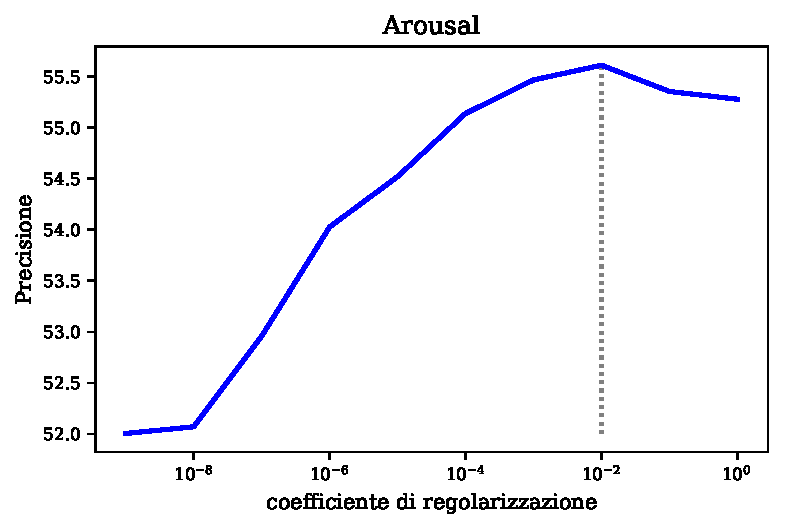
\includegraphics[width=.45\textwidth]{img/reg_coef_aro.pdf} & 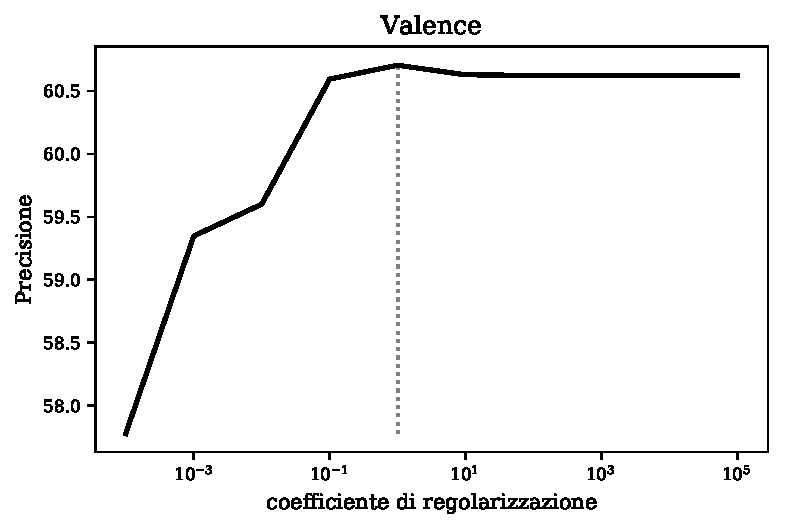
\includegraphics[width=.45\textwidth]{img/reg_coef_val.pdf}
\end{tabular}
\caption{Variazione della precisione di classificazione al variare del coefficiente di regolarizzazione. I valori ottimali sono indicati dalla linea verticale e sono rispettivamente $10^{-2}$ per l'arousal e $10^{-1}$ per la valence}
\label{img:regolarization_test}
\end{figure}


La stessa tipologia di classificatore è stato poi allenato e testato considerando solo le feature selezionate automaticamente con le seguenti tecniche:

\subsubsection{$KBest$}


\subsubsection{$Percentile$}


\subsubsection{$RFECV$}


La tabella \cite{table:feature_selection_table} mostra i risultati ottenuti dei diversi classificatori